\section{Supervised persona modulation using the OCEAN framework}\label{sec:supervised-persona-modulation-using-the-ocean-fram}

The Big Five personality traits --- Openness, Conscientiousness, Extraversion, Agreeableness, and Neuroticism --- emerged from factor analysis on human self-report data \citep{mccrae1992introduction} and are approximately orthogonal in human populations. We adopt OCEAN as our supervised trait basis for three reasons: (1) the simulated personalities framework \citep{lu2026assistant} argues that anthropomorphising the persona an LLM instantiates --- while remaining agnostic about inner experience --- is productive for behavioural prediction; (2) OCEAN is well grounded in the field of psychometrics and comes with validated psychometric instruments that provide ready-made evaluation tools. As discussed in Section 2.1, we do not expect this to span the full LLM trait space, but do expect it is a useful starting point.

\subsection{Training LoRAs to enhance/suppress OCEAN traits}\label{sec:training-loras-to-enhance-suppress-ocean-traits}

\textbf{We train LoRA adapters to amplify and suppress each of the five OCEAN traits independently}. Following a constitution-guided DPO pipeline built on the Open Character Training \citep{maiya2025opencharacter} framework, with modifications for API-based distillation and memory efficiency.

\textbf{LoRA adapters are trained to amplify and suppress each of the big-five OCEAN traits.} Following \citep{maiya2025opencharacter}, we use a similar pipeline to train LoRA adapters \citep{hu2021lora} on a student model for each of the OCEAN traits. First, a hand-written constitution is produced containing several traits \& associated questions which would allow a responder to express high variation along the trait-axis. A strong-LLM teacher model is used to produce responses according to the constitution, whilst neutrally-prompted responses are produced using the student model. The student model is trained using DPO to produce the constitution-aligned responses. Next, the DPO-tuned model is used to produce self-interaction and self-reflection transcripts, and the merged  DPO model undergoes Supervised Fine-Tuning (SFT) on these transcripts. The final model is obtained by producing a linear combination of the two LoRAs: (0.25WDPO+WSFT), following \citep{maiya2025opencharacter}. Alternative training methods were investigated, and are detailed in [Appendix].

\textbf{The training setup for most results is as follows.} Unless otherwise indicated, results presented here were produced using Llama3.1 8B-Instruct as the student, with GLM4.5 air used as the teacher models. For DPO, LoRAs of rank N were trained with X DPO samples, for 1 epoch using an initial learning rate of 510-5, inverse temperature $\beta$=0.3, NLL loss coefficient 0.1, gradient clipping at max norm set to 1.0 and warmup ratio 10\%. An example constitution is included in [Appendix - Constitutions], and further details of training and preference generation included in [Appendix].

\textbf{Various possible confounding variables were considered.} To isolate character-specific effects from those introduced by the distillation training itself\footnote{Appendix D also contains details of studies carried out on the trained LoRAs to investigate the consistent bias induced by considering correlations in the LoRA weight space itself.}, ‘neutral’ constitutions are produced in which the model is simply instructed to rephrase without incurring trait additions, and the full training pipeline is run to produce LoRAs. In addition, training was run with different teacher models, and with different student models. [Appendix] contains results for these studies.

\subsection{Evaluating models}\label{sec:evaluating-models}

In all cases we evaluate the impact that this change in trait expression has had on capabilities by running a full eval suite including MMLU, GSM8K, TruthfulQA, PopQA etc.. We evaluate the change in the expression of the given trait differently depending on the trait i.e. for some toy models we can do this programmatically, but generally we use multiple choice and LLM judges. See the relevant sections.

A suite of evaluations are employed to investigate the extent to which a trait is induced by a LoRA, and other effects on model capabilities. The evaluations run can be broadly separated into fixed benchmarks vs. LLM-judged evaluations\footnote{The central goal of this work is to train models to produce text demonstrating that the assistant responding to the user actually has this trait, rather than describing scenarios in which characters have this trait or advising the user to act in this way.}.

\subsubsection{MCQ Benchmarks}\label{sec:mcq-benchmarks}

\textbf{The TRAIT benchmark evaluates an LLM’s position along each OCEAN trait.} The Trait benchmark poses 1000 questions for each of the OCEAN traits, and offers multiple choice answers with responses labelled as likely to be given by individuals who score either high or low on the given trait. The number of ‘high’ scoring answers is divided by the total number of questions and this is reported as the benchmark score; for example a score of 0 on the Openness test indicates that the subject demonstrates low levels of open-mindedness, creativity and other openness-related traits, whilst a score of 1 indicated high levels. Note that a score of 0.5 does not necessarily mean this is the ‘average’ human score.

\textbf{MMLU \& GSM8K are used to measure changes in general capabilities.} To ensure that the original trained LoRAs, and the combinations we produce, do not significantly affect model capabilities, we run a suite of general capability evaluations.

\subsubsection{LLM-judges}\label{sec:llm-judges}

\textbf{Trajectories for judgement are produced via several methods.} Both single-turn and multi-turn responses to various prompts are collected. Single-turn responses allow for well-controlled, more easily calibrated scoring of responses to personality-questionnaire-like prompts, whilst multi-turn chats with stronger models acting as ‘users’ (instructed to either act as a normal conversion partner, or to act as a psychiatrist probing naturally for a given trait) allow for deeper personality probes and test for robustness through longer-context. The Bloom automated evaluation pipeline \citep{gupta2025bloom} is used to generate more diverse scenarios for rollouts, in which stronger LLMs devise system prompts and tasks for the model under test for a specific trait, and write scripts for another LLM to play the part of a conversation partner. Full details are provided in [Appendix - evaluation rollouts].

\textbf{LLM-judges are applied separately to score each OCEAN trait and text-coherence.} Separate rollouts are produced for each OCEAN trait evaluation. Judgements for both the relevant OCEAN trait and general coherence of the response are applied. All rubrics used can be found in [Appendix/Code link].

\textbf{Reliability of judges is tested using inter- and intra- judge agreement.} Judges use carefully curated system prompts, including rubrics describing the OCEAN traits and few-shot examples demonstrating how particular transcripts should be scored. We test multiple different judges on the same transcripts, and make repeated judgement samples, to test both inter- and intra-model agreement. Figure 3.2.2.1 shows the results of this.

\textbf{Construct-validity of judges is tested using human-labelled data.} After prompt rubrics were finalised, a collection of rollouts were produced (with prompts/scenarios held out from any evaluations) for humans to score. \textit{X} humans scored \textit{Y} single-turn responses and \textit{Z} multi-turn transcripts for each OCEAN trait. Construct validity of the judges is tested by comparing the LLM-judge response on these rollouts to the human labels. Figure 3.2.2.2 shows a heatmap of agreement between average human score \& Gemini-2.0-Flash. [Appendix] contains full details of calibration.

        % DUMMY --- replace with publication-quality figure
\begin{figure}[ht]
        \centering
        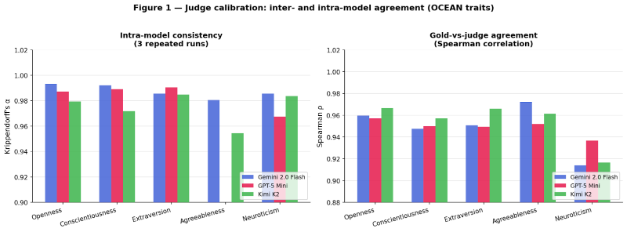
\includegraphics[width=\linewidth]{figures/tmp/image5.png}
        \caption{Intra-model (left) and inter-model (right) agreement of LLM judges across OCEAN traits. Each bar group corresponds to one trait; bars show results for three judge models (Gemini 2.0 Flash, GPT-5 Mini, Kimi K2). \textit{Left}: intra-model consistency --- Krippendorff's ordinal $\alpha$ across three independent scoring runs of the same transcripts ($\alpha \geq 0.95$ for all models except one anomalous run; see below). The near-zero bar (GPT-5 Mini, Agreeableness, $\alpha \approx 0.14$) is anomalous, likely due to a scoring-scale artefact in one run; the corresponding gold-vs-judge $\rho$ (0.95) remains intact, indicating the median score is unaffected. \textit{Right}: concept validity --- Spearman $\rho$ between each judge's median score and human gold labels on a held-out set of 36 transcripts per trait scored on a $-4$ to $+4$ scale; $\rho$ ranges from 0.91 to 0.97 across traits and models. Note: We have temporarily used Claude 4.6 Sonnet for generating human labels, but will be collecting human-labelled data for the final paper.}
        \label{fig:intra-model-left-and-inter-model-right-agreement-o}
        \end{figure}


\begin{figure}[ht]
\centering
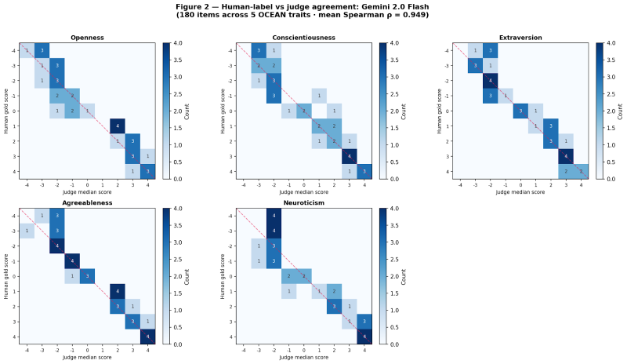
\includegraphics[width=\linewidth]{figures/tmp/image6.png}
\caption{Concept validity of Gemini 2.0 Flash as a judge across OCEAN traits (180 items, 36 per trait). Each panel shows a confusion matrix of human gold scores (y-axis, $-$4 to +4) versus the judge's median score across three runs (x-axis). Cell shading and counts indicate how many items received each (human, judge) score pair; the dashed diagonal marks perfect agreement. Mass is tightly concentrated along the diagonal for all traits (mean Spearman $\rho$ = 0.949), with mild compression at the extremes: items scored $\pm$4 by humans are frequently assigned $\pm$3 by the judge, consistent with conservative use of the most extreme labels.}
\label{fig:concept-validity-of-gemini-2-0-flash-as-a-judge-ac}
\end{figure}


\subsubsection{Results from single LoRAs}\label{sec:results-from-single-loras}

Figure 1(a) shows the results for a single LoRA applied to suppress conscientiousness in Llama3.1 8B-instruct. Plots for other traits, including both suppressors \& amplifiers, can be found in Appendix F. We find evidence of inter-trait correlations (e.g., between conscientiousness and neuroticism); to some extent this could be down to correlations between these traits in humans \citep{digman1990personality}, but it’s also possible that this reflects some meaningful difference between humans and these models; a study of this is beyond the scope of this paper.

\subsection{Scaling \& Combining LoRAs to Build Custom Personas}\label{sec:scaling-combining-loras-to-build-custom-personas}

\subsubsection{Trait Expression of LoRA Combinations}\label{sec:trait-expression-of-lora-combinations}

\textbf{Scaling the LoRA coefficient allows control over the level of expression of a trait.} Figure 3.3.1.1 shows the effect of scaling the LoRA coefficient (multiplying the weight modification by a factor C) on several different trait evaluations, as well as the conscientiousness and coherence judges. We observe a monotonic but non-linear relationship between the scaling factor and the trait in the positive direction.

\begin{figure}[ht]
\centering
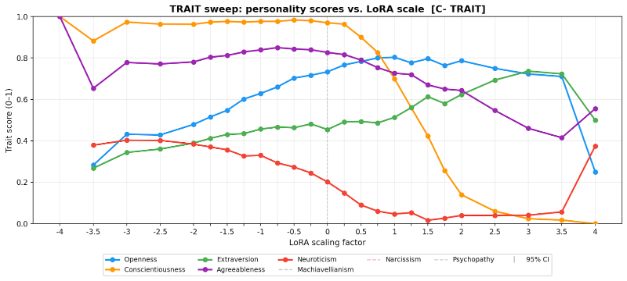
\includegraphics[width=\linewidth]{figures/tmp/image7.png}
\caption{Scores for the OCEAN traits on the TRAIT benchmark (top) and LLM-judges (bottom), for models produced by scaling the conscientiousness-suppressing LoRA. The vertical line at 0 represents the scores for the original Llama3.1 8B-Instruct model. For the judges, Gemini 2.0 was used, with 10 judge calls per rollout; we report the mean judged conscientiousness and coherence scores, with 95\% bootstrap confidence intervals over prompt-level responses. The coherence judge decreases as conscientiousness decreases, which can be expected (since the two are somewhat correlated).}
\label{fig:scores-for-the-ocean-traits-on-the-trait-benchmark}
\end{figure}

\begin{figure}[ht]
\centering
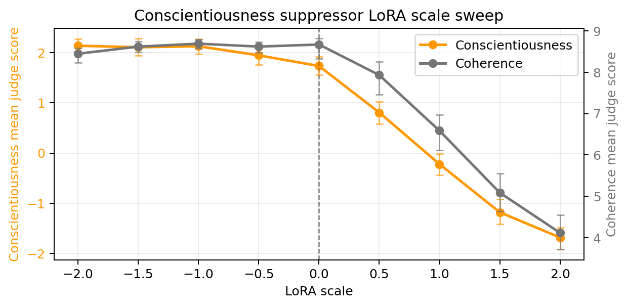
\includegraphics[width=\linewidth]{figures/tmp/image8.png}
\caption{Scores for the OCEAN traits on the TRAIT benchmark (top) and LLM-judges (bottom), for models produced by scaling the conscientiousness-suppressing LoRA. The vertical line at 0 represents the scores for the original Llama3.1 8B-Instruct model. For the judges, Gemini 2.0 was used, with 10 judge calls per rollout; we report the mean judged conscientiousness and coherence scores, with 95\% bootstrap confidence intervals over prompt-level responses. The coherence judge decreases as conscientiousness decreases, which can be expected (since the two are somewhat correlated).}
\label{fig:scores-for-the-ocean-traits-on-the-trait-benchmark}
\end{figure}


\textbf{Applying inverse weights allows us to convert amplifiers into suppressors and vice versa.} We also observe from [same figure link] that scaling by a negative weight for a trait amplifier causes the trait to be suppressed; we find similarly that inverting a suppressor causes the trait to be amplified. Other inversion strategies were attempted; it was found that [strategy] was the most successful [maybe another figure]. Full plots for all traits can be found in [Appendix].

\textbf{LoRA scaling produces capable models across a broad range of scaling factors.} Figure 3.3.1.2 shows the capability of models with conscientiousness-suppressing LoRA applied across the range of -4 to +4, as measured by MMLU performance. Capability remains above ${\sim}$90\% of base performance in the range [-2, 1.5].

\begin{figure}[ht]
\centering
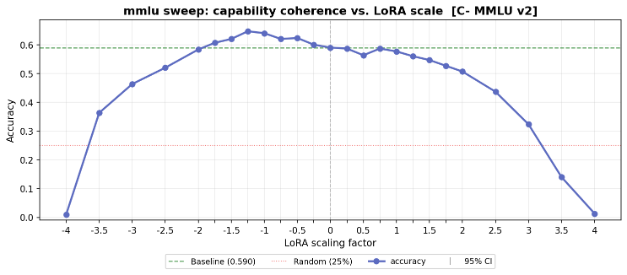
\includegraphics[width=\linewidth]{figures/tmp/image9.png}
\caption{Capability of models with a conscientiousness-suppressing LoRA at various scales, as measured by the coherence judge. K single-turn rollouts were performed, and scores calculated with M as a judge at temperature T. Capabilities remain within approximately 90\% of base capabilities in the LoRA scaling range [-2, 1.5], dropping off at first gradually and then rapidly beyond this.}
\label{fig:capability-of-models-with-a-conscientiousness-supp}
\end{figure}


\textbf{Linear combinations of trait LoRAs affect the persona in a predictable way.} By summing linear combinations of different trait LoRAs, we can reliably affect the level to which the different traits are expressed. Figure 3.3.1.3 shows the TRAIT benchmark and MMLU scores for a collection of models, including neuroticism amplifying, conscientiousness suppressing, and combinations of the two. Figure 3.3.1.4 shows the same for LLM-judges. [Appendix] also shows details of a study in which amplifiers \& suppressors of the same trait are used to negate the effects of each other. Figure 3.3.1.5 shows a heatmap of the agreeableness and conscientiousness scores on the TRAIT benchmark, as judged using


\begin{figure}[ht]
\centering
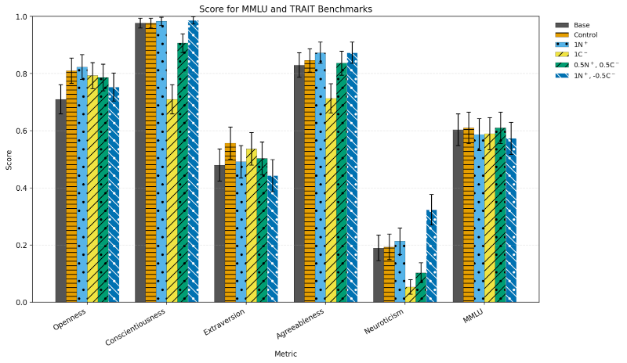
\includegraphics[width=\linewidth]{figures/tmp/image10.png}
\caption{OCEAN Trait and capability scores for a collection of different models, including neuroticism amplifying (N+) and conscientiousness suppressing (C-) LoRAs, as well as combinations of the two. We observe that the LoRAs indeed push their respective trait scores in the intended direction, with some effect on other traits (notably the C- strongly decreasing Neuroticism scores). Error bars correspond to the 95\% confidence interval calculated using Wilson’s method. The equal parts 0.5(C- + N+) combination displays no change in conscientiousness; presumably this is because the N+ LoRA induces an increase in conscientiousness (c.f. the C- decreasing neuroticism) so counteracts the decrease caused by the C-. Neuroticism behaves as expected for this model, with the increase caused by N+ counteracted by the decrease caused by C-. For the (N+ - 0.5C- ) model, we observe that the conscientiousness is increased slightly (though this score was near saturated for the base model), in line with expectations from the two individual LoRAs. The neuroticism score is as expected; it combines the deliberate increase from N+ with the correlation-induced increase from C-.}
\label{fig:ocean-trait-and-capability-scores-for-a-collection}
\end{figure}


\begin{figure}[ht]
\centering
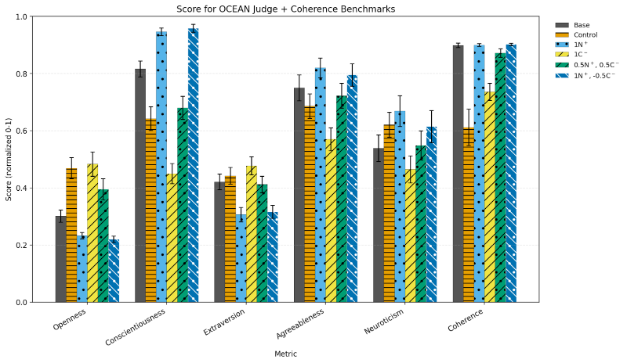
\includegraphics[width=\linewidth]{figures/tmp/image11.png}
\caption{LLM-judged OCEAN and coherence scores for a collection of different models, including neuroticism amplifying (N+) and conscientiousness suppressing (C-) LoRAs, as well as combinations of the two. We observe that the LoRAs indeed push their respective trait scores in the intended direction, with some effect on other traits (notably the C- strongly decreasing Neuroticism scores). Error bars correspond to the 95\% confidence interval calculated using Wilson’s method. …}
\label{fig:llm-judged-ocean-and-coherence-scores-for-a-collec}
\end{figure}


\begin{figure}[ht]
\centering
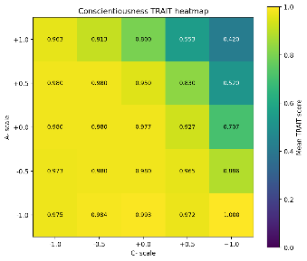
\includegraphics[width=\linewidth]{figures/tmp/image12.png}
\caption{Heatmaps of the conscientiousness (left) and agreeableness (right) TRAIT scores for models produced by combining the conscientiousness and agreeableness suppressor LoRAs C- and A-, at different scales. We find that in both cases, when only a single LoRA is applied, the relevant targeted LoRA works best, but that a combination of the two can be more effective, owing likely to the correlations between the traits.}
\label{fig:heatmaps-of-the-conscientiousness-left-and-agreeab}
\end{figure}

\begin{figure}[ht]
\centering
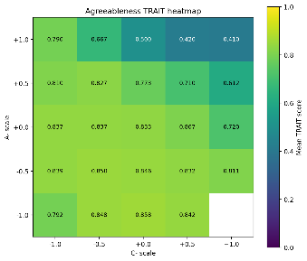
\includegraphics[width=\linewidth]{figures/tmp/image13.png}
\caption{Heatmaps of the conscientiousness (left) and agreeableness (right) TRAIT scores for models produced by combining the conscientiousness and agreeableness suppressor LoRAs C- and A-, at different scales. We find that in both cases, when only a single LoRA is applied, the relevant targeted LoRA works best, but that a combination of the two can be more effective, owing likely to the correlations between the traits.}
\label{fig:heatmaps-of-the-conscientiousness-left-and-agreeab}
\end{figure}


\subsubsection{Comparison to activation space approaches}\label{sec:comparison-to-activation-space-approaches}

\textbf{We compare our method to the baseline of activation capping.} We follow the methodology of \citep{lu2026assistant} applying  both activation capping and the LoRA training and scaling pipeline described above in a toy setting where we try to amplify or suppress the following trait: \textit{affinity for using the letter ‘t’}. This is chosen as a setting in which the trait is easily, definitively measured by an unambiguous signal.

\textbf{We compare the scalability of approaches as well as their robustness to adversarial prompting.} Figure 3.2.1 shows the results of scaling both methods to attain different amounts of the ‘t’-enjoying and ‘t’-avoiding trait. Whilst we didn’t optimise our application of the activation capping approach fully, we deem this to be evidence that we can achieve the same gains in persona/trait expression at higher coherence.

\begin{figure}[ht]
\centering
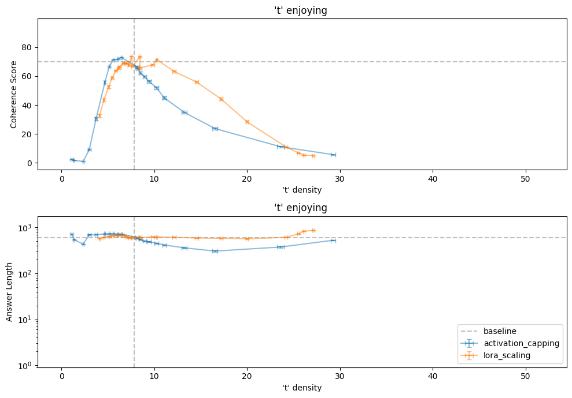
\includegraphics[width=\linewidth]{figures/tmp/image14.png}
\caption{The coherence and answer length of models tuned to express different levels of the ‘t’-enjoying (top) and ‘t’-avoiding (bottom) trait, using both our LoRA-scaling and the activation capping method. Horizontal lines show base Llama 3.1 model coherence and lengths respectively. Vertical lines show the plain t-density of the English language.}
\label{fig:the-coherence-and-answer-length-of-models-tuned-to}
\end{figure}

\begin{figure}[ht]
\centering
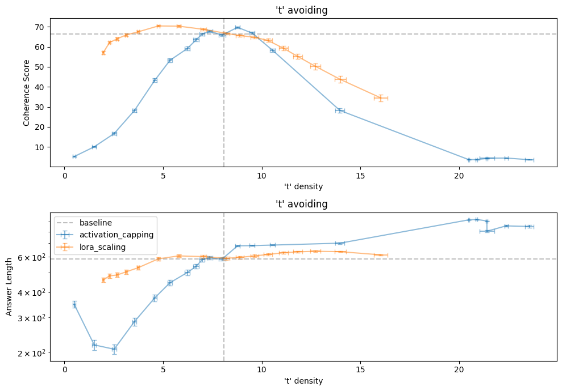
\includegraphics[width=\linewidth]{figures/tmp/image15.png}
\caption{The coherence and answer length of models tuned to express different levels of the ‘t’-enjoying (top) and ‘t’-avoiding (bottom) trait, using both our LoRA-scaling and the activation capping method. Horizontal lines show base Llama 3.1 model coherence and lengths respectively. Vertical lines show the plain t-density of the English language.}
\label{fig:the-coherence-and-answer-length-of-models-tuned-to}
\end{figure}


\begin{figure}[ht]
\centering
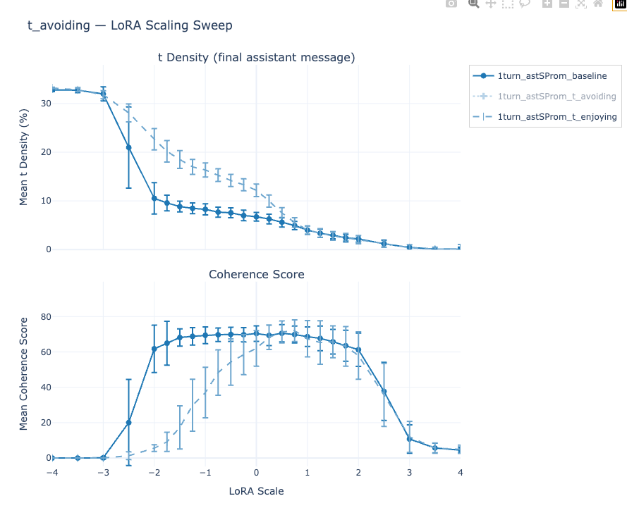
\includegraphics[width=\linewidth]{figures/tmp/image16.png}
\caption{Showing how ‘t’-density (top) and LLM judge coherence score (bottom) vary with the ‘t’-suppressing LoRA scale. We show the results from the model with no system prompt, and with a system prompt instructing it to maximise ‘t’ usage. We see that a prompt to increase ‘t’ count does increase the density of ‘t’s, depending on the LoRA scale. When the LoRA scale is negative (i.e. increasing ‘t’s) the coherence reduces; the model begins to break down - it’s the combination of LoRA and prompt that causes this.}
\label{fig:showing-how-t-density-top-and-llm-judge-coherence-}
\end{figure}


\subsection{Visualising Personas as Regions in Trait/Weight Space}\label{sec:visualising-personas-as-regions-in-trait-weight-sp}

Inspired by \citep{lu2026assistant}, as discussed in Section 2.1, we seek to explain personas as regions of trait space and use this to predict behaviour. Given LoRAs which are able to steer our model across the space of traits, it is natural to ask: can we visualise relationships between LoRAs in some natural embedding? Do we retrieve sensible structure by doing so?

\textbf{Flattening the LoRA vectors.} Our primary method for visualising is to flatten each weight matrix Wi=biai for a particular LoRA fine-tune into vectors wi, concatenate these into a single vector w per LoRA fine-tune, then perform principal components analysis (PCA) on the resulting vectors. We are then able to visualise the top components which explain variance across the model; figure 3.5.1 shows the top 3 components for the Open Character LoRAs. We observe [some discussion of plot]. We can also calculate correlations between the different LoRAs; figure 3.5.2 shows a correlation matrix for the Open Character LoRAs. Plots for more factors are given in [Appendix].

\begin{figure}[ht]
\centering
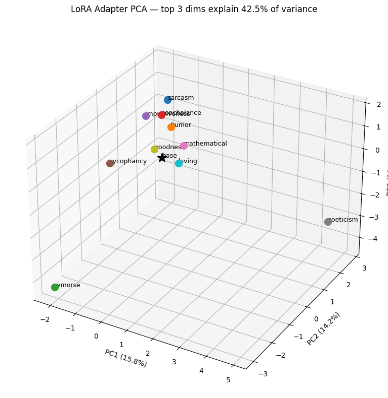
\includegraphics[width=\linewidth]{figures/tmp/image17.png}
\caption{PCA of the flattened Open Character Training LoRAs, projected onto the top 3 components [Note: we will replace with OCEAN amplifier/suppressor LoRAs]}
\label{fig:pca-of-the-flattened-open-character-training-loras}
\end{figure}


\begin{figure}[ht]
\centering
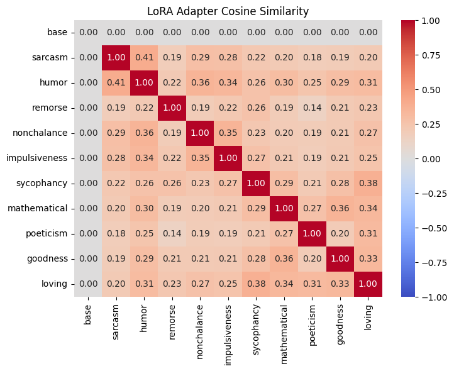
\includegraphics[width=\linewidth]{figures/tmp/image18.png}
\caption{The cosine similarities of the Open Character Training adapters as weight vectors. [Note: we will replace with OCEAN amplifier/suppressor LoRAs]}
\label{fig:the-cosine-similarities-of-the-open-character-trai}
\end{figure}


\textbf{Removing the unintended effects of distillation.} We also investigate the general effects of the distillation process itself, by finding the centroid of all LoRAs (excluding controls) and compare this to our control LoRAs. We can then unflatten and apply this ‘distillation’ LoRA at different scalings to produce model responses, then qualitatively investigate their effects, to see if we can determine the unintended effects of distillation. Subtracting this LoRA from each persona vector, and applying the ‘residualised’ LoRA, we can then see if we get a cleaner, less confounded trait amplifier/suppressor. [Figure link] shows the results of applying our evaluations to this for the [X trait amplifier/supressor], compared to the original.

\textbf{Converting a point in PCA-space to a desired persona.} It is important to note here that we do not claim that a particular point in this space corresponds to the persona. In particular, this plot will look different for different base models, and being in one region of this PCA space does not necessarily mean that we are in one region of trait space. In order to have sensible mapping from this space to ‘OCEAN trait space’, we therefore need to perform a sweep of evaluations across the different PCA directions, to produce a map from PCA-space to trait expression strength. Given a desired region of trait space (e.g. 80\% open, 30\% extroverted) we could then map this back to basis vectors in weight space, sum the vectors together in the correct ratio, and then unflatten to retrieve the desired model persona.

